\documentclass{beamer}
\usefonttheme[onlymath]{serif}
\usepackage[english]{babel}							%For internationalization
\usepackage[utf8]{inputenc}							%For character encoding
\usepackage{amsmath}								%For mathematical typesetting
\usepackage{amssymb}								%For mathematical typesetting
\usepackage{graphicx}								%For handling graphics

\newcommand{\be}{\begin{equation}}
\newcommand{\ben}[1]{\begin{equation}\label{#1}}
\newcommand{\ee}{\end{equation}}

\title
{An Introduction to Discontinuous Galerkin Methods}
\subtitle{Module 1: What is DG?}
\author[Bevan] % (optional, for multiple authors)
{J.~Bevan}
\institute[UMass Lowell] % (optional)
{
  Department of Mechanical Engineering, Grad Student\\
  University of Massachusetts at Lowell
}
\date[Fall 2014] % (optional)
{}
\subject{Discontinuous Galerkin}

\begin{document}
\frame{\titlepage}
\frame{\frametitle{Module 1: What is DG?}\tableofcontents} 
%NEW SECTION
\section{Overall Content Structure}
\subsection{Assumed Prerequisite Knowledge}
\frame{\frametitle{\textbf{\secname}: \subsecname}
\begin{itemize}
\item It is assumed the interested viewer is an advanced undergrad or graduate student with the typical STEM background of Calculus, Linear Algebra, and ODEs/PDEs.
\item Additionally, it is assumed the viewer has at least a basic background in a programming language of their choice (Matlab etc.)
\item Finally it is assumed the viewer has taken a general Numerical Methods course as well a Solution of PDEs course.
\item Not intended to teach common underlying techniques (interpolation etc.), but we may [Recall] important features of them.
\end{itemize} 
}

\subsection{Numerical Methods Prerequisites} 
\frame[shrink]{\frametitle{\subsecname}
\begin{itemize}
\item Linear algebra
	\begin{itemize}
	\item Vector spaces, bases, properties, etc.
	\item Orthogonality
	\item maybe some useful spaces (Hilbert, square integrable, etc)?
	\end{itemize}
\item Polynomial interpolation(1 and 2D)
	\begin{itemize}
	\item Lagrange, Hermite
	\item monomial basis (and ill-conditioned nature)
	\item Orthogonal basis (Legendre, Chebyshev)
	\item L2 projection
	\item choice of interpolation points (equispaced, GL, LGL, etc)
	\item Runge phenomenon
	\item Vandermonde matrix (transformation from modal to nodal spaces)
	\end{itemize} 
\item Quadrature (1 and 2D)
	\begin{itemize}
		\item Newton-Cotes
	\item Gauss/Hermite(Legendre)
	\item relation to interpolation

	\end{itemize} 
\item Solution of ODEs
	\begin{itemize}
	\item Forward Euler
	\item RK4
	\item Implicit schemes (e.g. Backward Euler)
	\item Stability, Convergence
	\end{itemize} 
\end{itemize} 
}

\subsection{Solution of PDEs Prerequisites} 
\frame[shrink]{\frametitle{\subsecname}
\begin{itemize}
\item Domain representation
	\begin{itemize}
	\item meshing
	\item BCs (Neumann and Dirichlet)
	\end{itemize}
\item Finite difference methods (FDM)
	\begin{itemize}
	\item Pointwise spatial derivatives
	\item Computational vs Physical domains
	\item Basic mapping (bilinear)
	\end{itemize} 
\item Finite volume methods (FVM)
	\begin{itemize}
	\item Flux functions
	\item Artificial viscosity
	\item Linear vs nonlinear fluxes
	\end{itemize} 
\item Finite element methods (FEM)
	\begin{itemize}
	\item Weak and strong form formulation
	\item Piecewise linear solution approximation
	\item Galerkin style test functions
	\item local support
	\end{itemize} 
\end{itemize}
}

\subsection{Lecture Goals} 
\frame[shrink]{\frametitle{\subsecname}
\begin{itemize}
\item Understand DG spatial discretization (advective)
\begin{itemize}
\item DG weak form (test function to minimize residual or test function orthogonal)
\item solution approximation (and initial conditions)
\item mapping physical to computation domain (for curvilinear domains)
\item DG Galerkin formulation
\item Integration by parts $\rightarrow$ flux functions (solution smoothness requirements): differences from FEM
\item linear vs non-linear flux: ramifications for semi-discrete system
\item hyperbolic vs parabolic
\item applying BCs (include periodic BCs)
\end{itemize}
\item  Understand time discretization
\begin{itemize}
\item Method of lines style semi-discrete form
\item Types: e.g. Forward Euler, RK4
\item CFL condition and stability
\end{itemize} 
\item Learn how to apply DG to arbitrary PDEs and realm of applicability
\begin{itemize}
\item intuitive understanding of methodology
\item conceptualization of process (not tied down to specific examples)
\item understand pros/cons
\item understand how DG “simplifies” to FVM and FEM
\end{itemize} 
\item Generate runnable code of your own
\begin{itemize}
\item Self-contained set of knowledge and algorithms to be able to write a full solver
\end{itemize} 
\end{itemize}
}

\subsection{Topics Layout} 
\frame{\frametitle{\subsecname}
\textbf{Module 1: What is DG?}\\
DG motivation (why vs FEM, FVM, FDM)\\
Scalar conservation law (linear) PDE\\
Weak form derivation\\
Global domain vs local element\\
Multiple-valued element boundaries\\
Recall: Flux functions\\
}

\frame{\frametitle{\subsecname (cont.)}
\textbf{Module 2: A Simple 1D DG Solver}\\
Linear solution approximation\\
Test function choice (Galerkin)\\
Upwind flux\\
Mass Matrix\\
Stiffness Matrix\\
Putting it all together (linear system)\\
Semi-discrete system\\
Forward Euler\\
Investigate h-convergence\\
Investigate t-convergence\\
Investigate stability (CFL)\\
}

\frame{\frametitle{\subsecname (cont.)}
\textbf{Module 3: To Higher-Orders (nodal) }\\
\textbf{3A: Sol’n Approximation}\\
Revisit weak form\\
-Approx. space\\
-L2 Projection minimizes residual norm\\
-Test space $\rightarrow$ orthogonal\\
Monomial basis?\\
Ill-conditioning of monomials\\
Recall: Lagrange interpolation (code)\\
Derive Lagrange spatial approximation\\
Equispaced interp points?\\
Runge phenomenon\\
Why: Bernstein/Markov inequality\\
Roots of Leg instead\\
}

\frame{\frametitle{\subsecname (cont.)}
\textbf{Module 3: To Higher-Orders (nodal) }\\
\textbf{3B: Discrete System}\\
Numerical Quadrature (Gauss)\\
Hermite interpolation (2N+1 quad)\\
Truncation error/exact quadrature\\
GL Lagrange orthogonality\\
Local Mapping Fun\\
Mass Integral ->diagonal/inversion\\
Log differentiation\\
Flux interpolation\\
Stiffness Integral\\
Numerical Flux (interpolated)\\
Assembly of system\\
RK4 time discretization\\
Investigate p-convergence (smoothness reqs)\\
}

\subsection{A Pedagogical Comment} 
\frame{\frametitle{\subsecname}
\begin{itemize}
\item Take advantage of format: replay, pause, speed up, slow down
\item Each section may have subsections, but the overall section is intended to be a self-contained concept. The first slide of a new section has the title format \textbf{Section}: Subsection
\item Easy to "zone-out", before the start of a new section try and put what you learned into action. Make a code snippet to test your understanding or verify a claimed result etc.
\item Each Module has a larger self-contained concept. You should be able to put together a script that accomplishes something substantial.
\end{itemize} 
}

%NEW SECTION
\section{DG Motivation: Why DG?} 
\frame{\frametitle{\textbf{\secname}}
\begin{itemize}
\item Overall purpose: PDE models physical system, solve PDE numerically
\item Compare to common techniques FDM, FEM, FVM:
\item Increasing order of solution can be more efficient, smooth functions especially. Most comm. packages low order (LO)
\item FDM not explicitly conservative, extended stencil for high order (HO) a problem for unstructured grids
\item FEM not good for hyperbolic problems, discontinuities in sol'n troublesome
\item FVM constant solution of volume necessitates extended stencil for HO, ruins flexibility for unstructured grids
\item DG is explicitly conservative, well-suited for hyperbolic problems, able to handle discontinuities, and can still use unstructured grids at HO
\item Local nature of solution permits good parallelizability
\item Can use numerical flux functions to capture physical behavior
\end{itemize} 
}

%NEW SECTION
\section{Example PDE: Scalar Conservation Law}
\subsection{A brief motivating example}
\frame[shrink]{\frametitle{\textbf{\secname}: \subsecname}
Imagine some scalar quantity that is subject to a conservation law
\begin{figure}
\centering
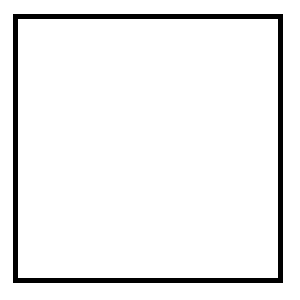
\includegraphics[width=.5\textwidth]{square.PNG}
\end{figure}
}
\subsection{General Approach}  
\frame{\frametitle{\subsecname}
\begin{itemize}
\item As worked out, PDE for system in 1D is
\be \frac{\partial q}{\partial t} + \frac{\partial f(q)}{\partial x} = S(x) \ee
\item We will need to decide how we solve this system, and we will need to discretize in space and time
\item The first term will be discretized with a Forward Euler approach, the second term will be handled by DG
\item For simplicity we assume no sources, and a linear flux with an externally prescribed velocity field
\end{itemize} 
}

%NEW SECTION
\section{The Weak Form of the PDE} 
\frame{\frametitle{\textbf{\secname}}
\begin{itemize}
\item We will discuss the finer points of this in Module 3, for now permit the following; the weak form solution of the PDE is the integral (over the global domain $\Omega$) of our solution times some test function $\phi$:
\be \int_{\Omega} \frac{\partial q}{\partial t} \phi \,dx + \int_{\Omega} \frac{\partial f(q)}{\partial x} \phi \,dx = 0 \ee
\item In DG the global domain is split into K elements, where the local sol'n is defined for a particular element. The global sol'n is then the direct sum of each of these local polynomials, a piecewise polynomial
\item This is similar to a FEM approach, however continuity is not enforced across elements
\end{itemize}
}

%NEW SECTION
\section{Domain Decomposition: Global vs Local} 
\frame{\frametitle{\textbf{\secname}}
\begin{itemize}
\item The integration domain is now over the element instead of the whole domain such that $\{x|x \in k, x_L \leq x \leq x_R\}$
\item To reduce smoothness requirements on the flux we integrate the second term by parts to get
\be \int_k\! \frac{\partial q}{\partial t} \,\phi \,dx +
	[f(q)\phi] \Big\rvert_{x_L}^{x_{R}} -
	\int_k\! f(q) \,\frac{d\phi}{dx} \,dx = 0 \ee
\item Notice that we include the endpoints of our domain $k$
\item Endpoints of neighboring elements are coincident, so $q$ is multiply defined, what ramifications does this have? Also, we now have K independent local solutions, how do we recover the global solution?
\end{itemize}
}

%NEW SECTION
\section{Element Boundaries: Multiply Defined?} 
\frame{\frametitle{\textbf{\secname}}
\begin{itemize}
\item If $q$ is multiply defined at endpoints, what should $f(q)$ be?
\item In order to ensure conservation flux between elements should be equal $-f_{k-1}(q(x_R)) = f_{k}(q(x_L))$
\item Take a FVM approach and permit a \textit{numerical flux} denoted $\hat{f}(q)$
\item The numerical flux function permits communication between elements, allowing recovery of global sol'n
\end{itemize}
}

%NEW SECTION
\section{[Recall] Flux Functions} 
\frame{\frametitle{\textbf{\secname}}
\begin{itemize}
\item Flux functions describe the "flow" of some quantity depending on the quantity itself and possibly other factors
\item Permits insertion of problem specific knowledge into an otherwise agnostic PDE
\item Many choices, Lax-Friedrichs, Richtmyer, Godunov, Osher, Roe, etc.
\item For simplicity we will use the upwind flux where $\hat{f}(q^+,q^-)=cq^-$ if $c>0$ and $cq^+$ if $c<0$
\end{itemize}
\begin{figure}
\centering
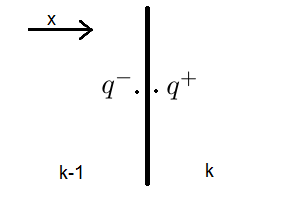
\includegraphics[width=.35\textwidth]{qBoundary.PNG}
\end{figure}

}

\end{document}